\vspace{-1cm}
\begin{wrapfigure}[15]{r}{7cm}
  \centering
  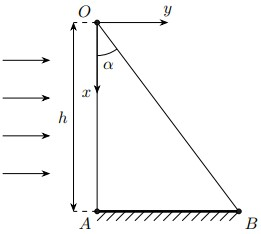
\includegraphics[width=0.38\textwidth]{Figures/Fig 5.jpg}
  \begin{center}
    \figurename{ 5}
  \end{center}
\end{wrapfigure}

\noindent Nhà thí nghiệm Gluck đã tiến hành một thí nghiệm quang học sử dụng một lăng kính đặc có tiết diện mặt cắt là tam giác vuông $OAB$ với các cạnh góc vuông là $AB$ và $OA=h$. Tất cả các mặt của lăng kính đều song song hoặc vuông góc với mặt phẳng hình vẽ. Nếu ta sử dụng hệ toạ độ $Oxy$ như được chỉ ra trên hình $5$, chiết suất của vật liệu làm lăng kính thay đổi theo công thức:
\begin{equation*}
  n(x)=\frac{3}{2-\dfrac{x}{h}}
\end{equation*}
Gluck quyết định chiếu một chùm sáng song song lên mặt bên $OA$ của lăng kính. Mặt đáy $AB$ được phủ một lớp vật liệu có khả năng hấp thụ toàn bộ ánh sáng đi qua nó. Lăng kính được đặt trong không khí, giả sử chiết suất của không khí bằng 1. Chỉ xét có tia sáng đi vào lăng kính thông qua mặt bên $OA$.
\begin{enumerate}
  \item Xét một tia sáng đi vào lăng kính tại điểm có toạ độ $x_{0}$. Xác định phương trình quỹ đạo của tia sáng đó bên trong lăng kính.
  \item Với những giá trị nào của góc $\hat{AOB}=\alpha$, các tia sáng sẽ đi qua mọi điểm trên mặt bên $OB$ của lăng kính?
  \item Với những giá trị nào của góc $\alpha$, tất cả các tia sáng khi đạt tới mặt bên $OB$ của lăng kính đều bị khúc xạ và đi ra không khí?
\end{enumerate}